\documentclass[letterpaper,10pt]{article}
\usepackage{fullpage}
\usepackage{authblk}
\usepackage{abstract}
\usepackage{appendix}
\usepackage{subcaption}
\usepackage{xspace}
\usepackage{graphicx}
\usepackage{amsmath,amssymb}
\usepackage{xcolor}
\usepackage{url}
%\usepackage{algorithm}

% algorithm stuff
\usepackage[noend]{algpseudocode}
\usepackage[ruled, vlined]{algorithm2e}
\newcommand{\myalgorithm}{
\SetKwProg{Procedure}{Procedure}{}{}
\SetKwProg{Function}{Function}{}{}
\SetKwProg{Iblock}{}{}{}
\DontPrintSemicolon
}
\newcommand\mycommfont[1]{\footnotesize\ttfamily\textcolor{blue}{#1}}
\SetCommentSty{mycommfont}


\makeatletter
\renewcommand\AB@affilsepx{, \protect\Affilfont}
\makeatother

\newtheorem{property}{Property}


\newcommand{\LBFT}{LBFT\xspace}
\newcommand{\PP}{\ensuremath{\mathbb{P}}\xspace}
\newcommand{\rust}[1]{\ensuremath{\mathtt{#1}}\xspace}
\newcommand{\module}[1]{\textcolor{orange}{\ensuremath{\mathbf{\mathsf{#1}}}\xspace}}
\newcommand{\preferred}{\rust{preferred\_round}}
\newcommand{\processcerts}{\rust{process\_certificates}}


\begin{document}
\title{Reconfiguration of the Libra Blockchain by Self-Reflecting Transactions}
\author{The LibraBFT Team}
\date{}
\maketitle

% **********************************************************************

\newcommand{\myomit}[1]{}

\begin{abstract}
This report describes reconfiguration of LibraBFT - an extension to \LBFT to support reconfigure itself
 by embedding configuration-change transactions in the sequence.
\LBFT addresses the fundamental consensus problem of the libra blockchain with fixed configuration setup,
think of validator set, consensus keys, VM features, software version etc.
Those are all like configuration of one \LBFT protocol instance. we want to support those configuration changes
without human intervention which could be excessive work and error prone. Instead we present
a protocol to handle reconfiguration just like a normal transaction.
\end{abstract}

\section{Introduction}
Reconfiguration of consensus protocol is not a new topic, it has been studies for decades and has more and more use cases in recent blockchain
area.

We'll present our mechanism to support reconfiguration of \LBFT in section \ref{mechanism}, and discuss the approches we considered and
comparison between them in section \ref{alternatives}, finally we'll give the correctness argument for all approaches in section \ref{correctness}.

At the high level, reconfiguration is under the authority of the current set of validators and operates via reconfig-transactions embedded inside the normal chain of transactions.
The chain continues beyond the reconfiguration transaction just like normal transactions, and the node should use the on-chain configuration to
spawn \LBFT instance. Genesis transaction is the first reconfiguration transaction and defines the configuration for the first \LBFT instance.

Epoch is the counter for the on-chain configurations, it's bumped after reconfiguration transactions. \LBFT instance is constructed with configuration
including epoch, ledger state, validator set etc. and initializes its internal state such as setting round to 0, generating genesis block for block store
etc. Blocks in different epochs are not chained and are internal to each \LBFT instance, but the underlying ledger state(chain of transactions) are continued.

\begin{figure}[ht]
	\centering
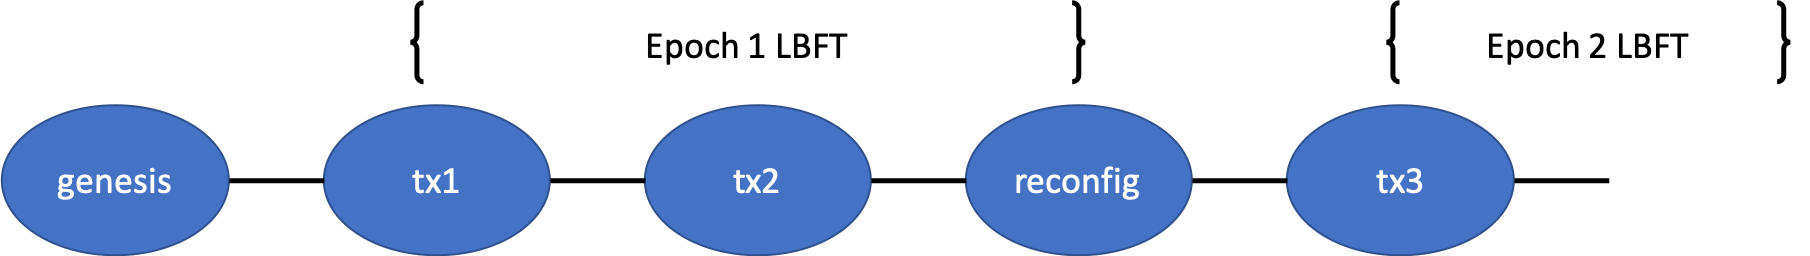
\includegraphics[scale=.45]{figures/introduction.png}
\caption{reconfiguraiton with multi LBFT instances}
\end{figure}

\section{Reconfiguration Mechanism} \label{mechanism}

In this section we describe the reconfiguration protocol and the changes required to \LBFT protocol.
One of the design goal is to decouple these two protocols as much as possible to provide nice abstractions.
\begin{figure}[h]
			\centering
		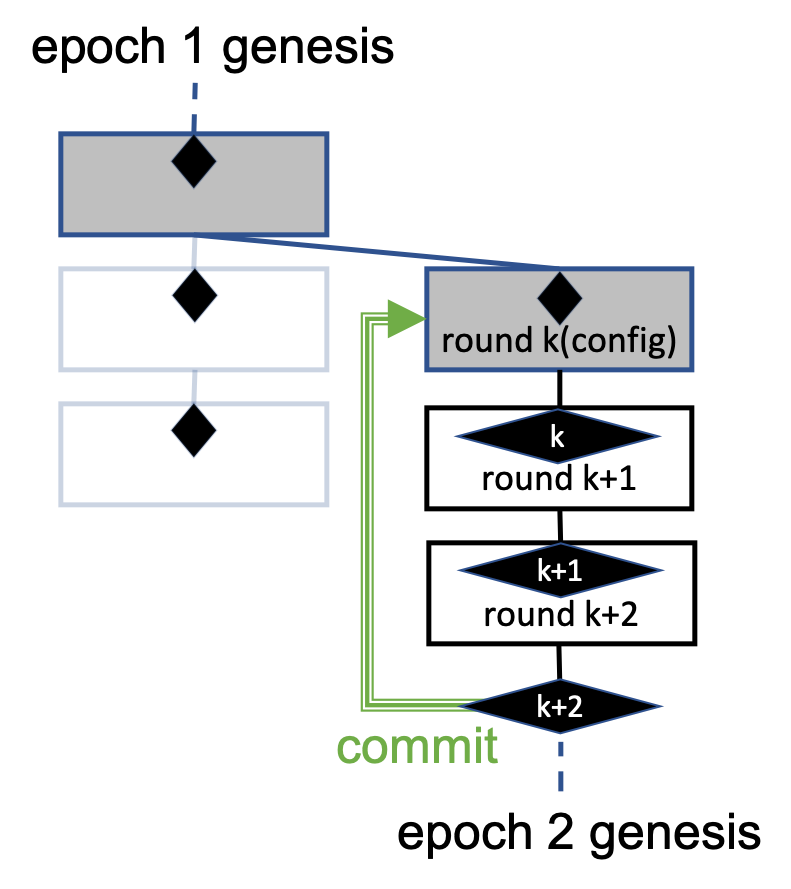
\includegraphics[scale=.45]{figures/reconfig1.png}
	\caption{Commit reconfig transaction}
\end{figure}

\subsection{Reconfiguration Protocol}

\emph{Epoch} is a monotonous increasing number used to refer to a \LBFT instance running with a specific configuration.
\LBFT instance is agnostic to epoch numbers, so we introduce \module{EpochManager} to process epoch related information.

\subsubsection{Message types}

First we add \emph{epoch} to every message types of \LBFT protocol including proposals, votes, timeout msg etc. Messages
with the same \emph{epoch} as local \LBFT protocol go to \LBFT for processing. Messages that have different \emph{epoch}
go to \rust{EpochManager.process\_different\_epoch\_messages}.

Additionally we introduce two messages types \rust{EpochChange} and \rust{EpochRetrieval}:

\begin{algorithm}[H]
\myalgorithm
{\SetAlgoNoLine
\tcp{The commit proof signed by \LBFT}
\Iblock{\rust{LedgerInfo}}{
	\rust{state\_id} ;\;
	\rust{signatures} ;\;
	... \;
	\rust{next\_configuration}: \rust{Option<Configuration>} ; \tcp{Added field to support reconfiguration}
}

\BlankLine
\tcp{Signals an \emph{epoch} change from $i$ to $j$}
\Iblock{\rust{EpochChange}}{
	\rust{start\_epoch} ; \tcp{The epoch of the first ledger info}
	\rust{end\_epoch} ; \tcp{The epoch after the last ledger info}
	\rust{proof}: \rust{Vec<LedgerInfo>} ;
}

\BlankLine
\tcp{Rquest an EpochChange from start\_epoch}
\Iblock{\rust{EpochRetrieval}}{
	\rust{start\_epoch} ;
}
}
\end{algorithm}

\subsubsection{EpochManager}
We have three different handlers for \module{EpochManager} to process those messages.

\paragraph{Handling different epoch, \rust{process\_different\_epoch\_msg}:}

When the different \LBFT epoch messages comes, we'll compare our local \emph{epoch} with the messages. If we're behind, we'll
issue a \rust{EpochRetrieval} to the peer who sent the message. If we're ahead, we'll provide
a \rust{EpochChange} to the peer.

\paragraph{Handling epoch retrieval, \rust{process\_epoch\_retrieval}:}
It's similar to how to process messages from lower \emph{epoch}, we'll provide the \rust{EpochChange} to help peer join our
\emph{epoch}.

\paragraph{Handling epoch change, \rust{start\_new\_epoch}:}

When we receive an \rust{EpochChange}, first we verify we're at \emph{epoch} $i$ and the \rust{EpochChange} is correct by iterating through the
ledger info and verify the signatures are corresponding to the configuration, then we ensure we're ready for the configuration of \emph{epoch}
$j$ e.g. sync to the ledger state at the beginning of the \emph{epoch} $j$. Finally we spawn a new \LBFT instance with
 the configuration of \emph{epoch} $j$.

\subsection{Changes to \LBFT}

Although \LBFT is agnostic to \emph{epoch}, it has to support additional rules for \textbf{reconfiguration protocol} in order to
maintain the safety property across \emph{epoch}.

\subsubsection{Commit Flow}
Just a kind reminder that \LBFT has three-phase commit rule - once we collects a QC for three contiguous rounds k, k+1, k+2, we commit the the block at round k
and all its prefix.

To support \rust{EpochChange} mentioned above, we need to add an optional field \rust{next\_configuration} to the \rust{ExecutedState}
which is only outputed when executing a reconfiguration transaction. Remember that \rust{LedgerInfo} carries the \rust{ExecutedState},
so that it contains such field and can serve as end-peoch proof.

Besides the normal commit flow in \LBFT which persists transactions in ledger state, we have an additional step to broadcast
\rust{EpochChange} to all the current validators if the \rust{LedgerInfo} carries next\_configuration. \module{EpochManager}
would then kick in and handle the \rust{EpochChange} message and spawn new \LBFT instance with next\_configuration and shutdown the current one.

\subsubsection{Descendants of Reconfig Block - Safety} \label{safety}

In this section, we explain the need to keep all the descendants of a reconfig-block empty of transactions until it's committed otherwise we might
have safety violation e.g. double spend.

The fundamental problem here is that \LBFT spreads the phase of the protocol(for every proposal) over 3 rounds i.e.\ pipelining.
When it comes to configuration, the proposal after reconfiguration transaction is under a different configuration with its
parent and the pipelining may not work anymore, we'll discuss more about this in section \ref{correctness}.

We use validators configuration as example, demonstrated in Figure~\ref{fig:safety}. Imagine we're at \emph{epoch} $1$ with
\rust{validators\{a1, a2, a3, a4\}}, and there's a reconfiguration transaction changes us to \rust{validators\{c1, c2, c3, c4\}}.
Reconfiguration transaction is included in B1, and a4 collects QC for B3 which has a ledger info(commit proof) of B1 but only unveils to \rust{c1,
c2, c3} but not \rust{a1, a2, a3}. \rust{c1, c2, c3} will start the new epoch and use B1 as its genesis while \rust{a1, a2, a3}
is going through another three rounds B4, B5, B6 and finally commit B4(which has B1 as its ancestor) and unveil it to \rust{c4}.
Now \rust{c4} thinks B4 is the genesis. If we have a double spend txn1, txn2 that txn1 committed with B4 and txn2 committed in B10 in
new \emph{epoch} $2$ with \rust{c1, c2, c3}, clients who query \rust{c1, c2, c3} would see the double spend compared with \rust{c4}.

\begin{figure}[ht]
			\centering
		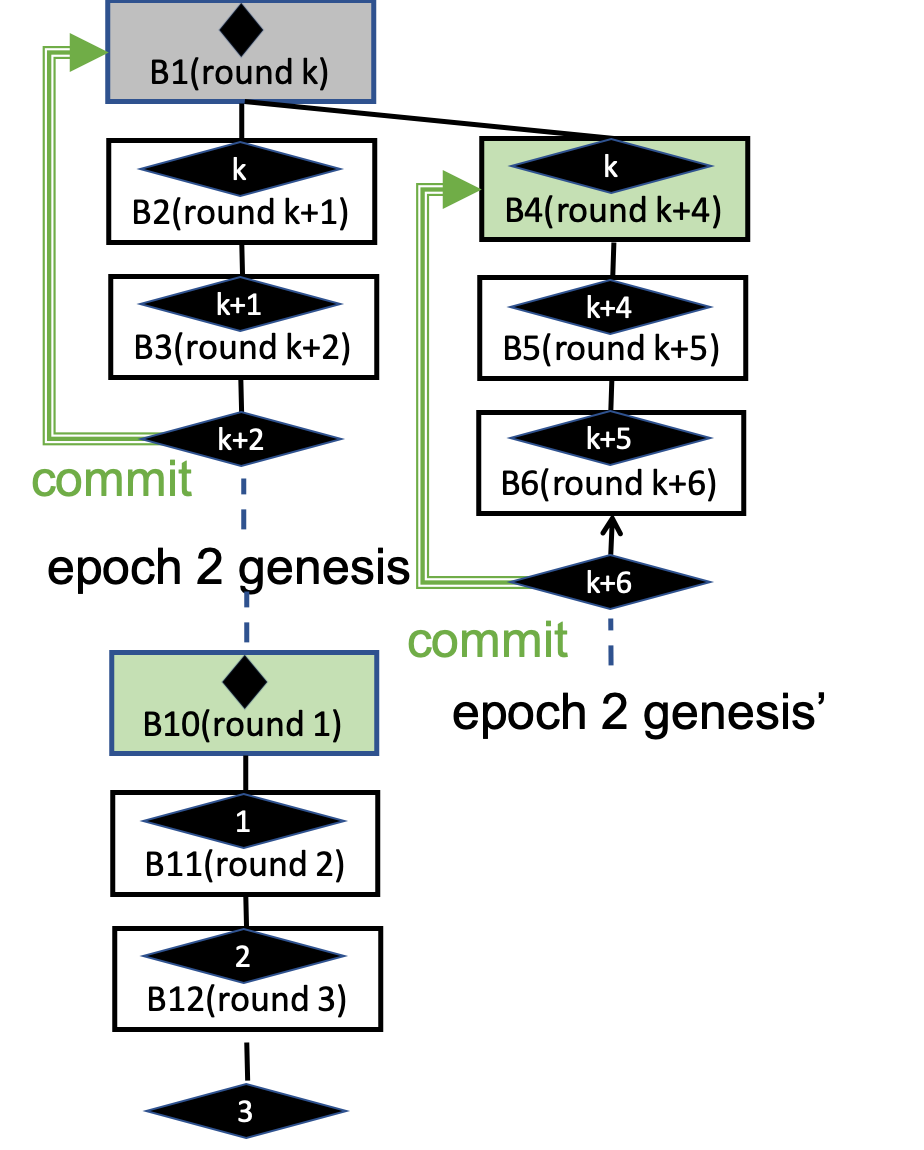
\includegraphics[scale=.45]{figures/reconfig-safety.png}
	\caption{Double spend in B4 and B10(green box)}
\label{fig:safety}
\end{figure}

Having any descendants of reconfiguration empty solves this problem, semantically it's equivalent to run 3 phases without
pipelining.

\subsubsection{Epoch Boundary - Liveness}
In this section, we explain how to specify the boundary of each \emph{epoch} and the risk of losing liveness if we don't do it correctly.
\paragraph{Start}
In \LBFT we assume everyone starts from a known genesis which we can consider as part of the configuration otherwise we'll lose liveness
even we preserve safety with empty blocks.
Intuitively we could use the block that includes reconfiguration transaction, but we may not commit that block directly but instead one
 of its descendants. And even worse, we may have multiple commit of its descendants since byzantine nodes could hide commits as Figure~\ref{fig:liveness}
 demonstrates.

\begin{figure}[ht]
	\centering
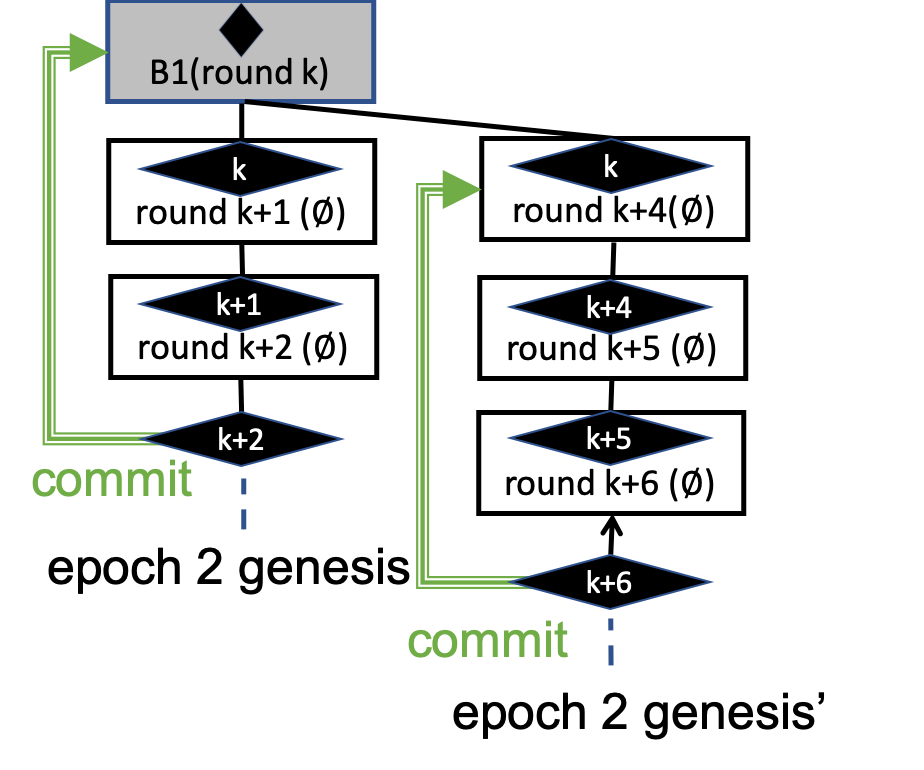
\includegraphics[scale=.45]{figures/reconfig-liveness.png}
\caption{If genesis is not equal to genesis', we lose liveness}
\label{fig:liveness}
\end{figure}

With the empty suffix blocks change, we ensure the same ledger state when we commit reconfiguration transaction regardless of which decendants,
and we leverage that to derive a genesis block so that every ledger info that ends previous \emph{epoch} would result in the same genesis deterministically.

\paragraph{End}
After a node sees \rust{LedgerInfo} that has \rust{next\_reconfiguration}, it'll stop participating the current \LBFT instance,
and spawning next \LBFT instance. If it's not part of the next reconfiguration, counterintuitively it can not shutdown itself
immediately otherwise we'll lose liveness. As an example, if we have \rust{validators\{a1, a2, a3, a4\}} at \emph{epoch} $i$, and
malicious \rust{a4} collects a \rust{LedgerInfo} and sends to \rust{a1} that's not part of \emph{epoch} $i+1$ and
\rust{a1} decides to shutdown itself. Byzantine node \rust{a4} also stops participating then \rust{a2, a3} would suffer a liveness problem and are never
able to make progress. To address such problem, \rust{a1} needs to keep the \rust{EpochManager} running until it sees a QuorumCert from new
\emph{epoch} so that it knows at least f+1 honest nodes in the new \emph{epoch} bootstrap.

\section{Alternatives} \label{alternatives}
In this section we briefly discuss some other approaches we considered for the problem and the trade offs.

\subsection{Quorum Compatible}
As we mentioned in \ref{safety}, we give up the pipeline of \LBFT to preserve safety. Here we consider an alternative that preserves
both safety and pipeline.

\paragraph{Condition}

Consider a reconfiguration transaction that changes from validators \rust{N1} to validators \rust{N2} and $f1=\lceil|N1|/3\rceil-1$,
$f2=\lceil|N2|/3\rceil-1$ malicious power, $|N1|-f1$,  $|N2|-f2$ as quorum size respectively. We only allow reconfiguration if

\begin{equation}
|N1 \cap N2| > f1 + f2 + max(f1, f2)
\end{equation}

\paragraph{Analysis}
We have an important lemma in \LBFT for safety: Under BFT assumption, for every two quorums of nodes, there exists an honest node that
belongs to both quorums.

With this approach, we restrict the changes between two configurations and we can prove quorums are interchangeable in both configurations,
so that we implicitly maintain the safety property.

\subsection{Pipelined Configuration}
This is one step further on top of the quorum compatible approach. Instead of implicit compatible quorums, we require explicit two quorums
to commit the reconfiguration transaction. We preserve the same safety lemma as above but doing it in a more explicit way.

One way to think about this is pipelining the reconfiguration like we pipeline blocks, reconfiguration $A\rightarrow B$ takes effect
(the next blocks on this branch need B’s quorum) right after the block and until a commit of another reconfiguration $B\rightarrow X$.

\subsection{Comparison}
We assemble a comparison table for the three approaches we describe.
\begin{table*}[h]
\begin{tabular}{|c|c|c|c|}

\hline
& Pipelining & Implementation Complexity & Flexibility\\
\hline \hline
Basic & No & Small & Most\\
Quorum Compatible & Yes & Medium & Least\\
Pipelined Configuration & Yes & Big & Medium\\
\hline

\end{tabular}
\end{table*}

Basic mechanim gives up pipelining/performance while provides more flexible configuration changes like protocol change, it also provides better
isolation between different configurations.

Quorum Compatible enables us with pipelining and is almost seamless to \LBFT by strictly limit how configuration can change.

Pipelined configuration provides pipelining the same as Quorum Compatible with more flexible reconfiguration by supporting explicit multi quorums.

Also regardless of implicit or explicit quorums, to support pipelining configuration, we need to track configuraiton per block tree branch which
adds complexity compared to one configuration per whole block tree in basic mechanism.

We chose the approach considered all above and think the performance gain of pipelining can not justify the added complexity and
lost flexibility for now, but could leave for future work.

\section{Correctness} \label{correctness}

It is useful to think about correctness in the following manner. Each round in the chain represents a slot in a sequence of consensus decisions.
Once a decision is committed, it takes effect immediately in the next slot. For normal transactions, this means that the state of the ledger is
updated by each slot, starting with the state of the previous slot. For control actions like reconfiguration, it changes the algorithm itself.
This again, takes effect in the immediate slot following the control transaction.
Generally, note that reconfiguration transactions can change any aspect of the algorithm, not just the validator set.

Now, imagine that an entire consensus algorithm is done separately for each round/slot. Clearly, to agree on the commit output of the algorithm
we must have agreement on the algorithm itself. Initially, the system is bootstrapped with an algorithm (and in particular, the
validator-configuration) responsible for slot 1 pre-determined and known to all via genesis transaction. Thereafter, if a slot commits an algorithm (configuration) change,
it takes effect in the succeeding slot.

It is fairly obvious to see inductively that in this manner, we maintain agreement on the algorithm for each slot.

\paragraph{Enters pipelining}

As depicted above under “Pipelined reconfiguration”, the DiemBFT consensus algorithm “spreads” the phases of the protocol (for every slot) over
3 rounds. More specifically, every phase is carried in a single round and contains a new proposal. For example, the leader of round k drives only
a single phase of certification of its proposal. In the next round, k+1, a leader again drives a single phase of certification. Interestingly,
this phase has multiple purposes:
\begin{itemize}
\item The k+1 leader sends its own k+1 proposal.
\item It also piggybacks the QC for the k proposal. In this way, certifying at round k+1 generates a QC for k+1, but also a QC-of-QC for k.
\item In the third round, k+2, the k proposal can become committed, the k+1 proposal can obtain a QC-of-QC, and the k+2 can obtain a QC.
\end{itemize}

Importantly, it should be understood that spreading phases of the k-protocol into rounds k+1 and k+2 does not shift the responsibility away from the k-algorithm.

To complicate matters, if any phase aborts due to a timeout, the k-protocol remains undecided. It can become committed only via a transaction that extends the k branch. If the k command is a reconfiguration command, the reconfiguration takes effect only upon the next commit.

For example, say that round k+1 aborts (no QC(k+1) obtained). The leader for k+2 extends k, and if three consecutive rounds (k+2, k+3, k+4) complete, then the prefix of the branch up to and include k+2 becomes committed, including k. Importantly, in this case, the reconfiguration transaction takes effect at round k+2.

A correctness “meta argument” reduction is the follows:

If the algorithm for a slot k is A, then it is necessary and sufficient for the quorums used for three slots succeeding the first commit on a branch extending A to contain quorums of A. If there is no gap, then rounds k, k+1 and k+2 use algorithm A. If there is a gap and k’ is the next commit, then rounds from k all the way to k’, k’+1, k’+2 use algorithm A.

If round k* (once committed) changes the configuration to A’, then similarly, it is necessary and sufficient for slots succeeding k* to contain quorums for A’ but also A until k* becomes committed.

\paragraph{Reconfiguration condition with pipelining}
Consider a round-k proposal such that:
\begin{itemize}
\item the last committed reconfiguration transaction on the branch which the k proposal extends is A (hence, A is “in effect”)
\item the k proposal changes (once committed) the algorithm from A to A’
\item k becomes committed by a round k* transaction which extends the k-branch
\end{itemize}
Then the following is necessary and sufficient for reconfiguration to not fork:
\begin{itemize}
\item A’ should take effect at round k+1
\item rounds k+1 thru k*+2 must use QC’s that contains quorums of both A and A’.
\end{itemize}

This “meta argument” suffices to show that the above proposals all work. The proposals differ in other properties they provide, such as ease of implementation, building state-transfer transition into reconfiguration, etc.


% **********************************************************************
\begingroup
\bibliographystyle{plain}
\bibliography{citations}
\endgroup

\end{document}
